\section{WC 9/6/25}

\subsection*{Overview:}this week I created a new Welcome page for users, redesigned my authentication pages, hugely optimised my code and implemented tools to help me monitor the status of my project enabling me to quickly respond to any issues.
\subsection*{Achievements, Thoughts and Ideas:}
I had initially approached this week aiming to launch my project to my waiting list and collect feedback however, during a gym session inspiration hit and came up with an artistic concept for a landing page for my project. Currently, when visitors access my website they see a login page straight away. Whilst this is functional and takes them straight to the end project it doesn't give much explanation to someone who had causally wondered into my project from the wider internet. To solve this I have built another webpage using my previous skills. 

This page features a randomly generating graph of nodes which represent the notes a user might create, I am very proud of this 3d visualisation as I learnt the framework required and implemented it into this product within a short amount of time. I have gone through a couple of iterations of this design, starting with more blue hues and eventually settling on a dark purple aesthetic which I am hugely found of.

This 'landing page' explains the project, its features and the motivations behind it. It also has a 'call-to-action' button which takes users to the login/registration page. Please see below for my first prototype and final version of this page.

\begin{figure}[H]
    \centering
    \begin{minipage}[b]{0.48\textwidth}
        \centering
        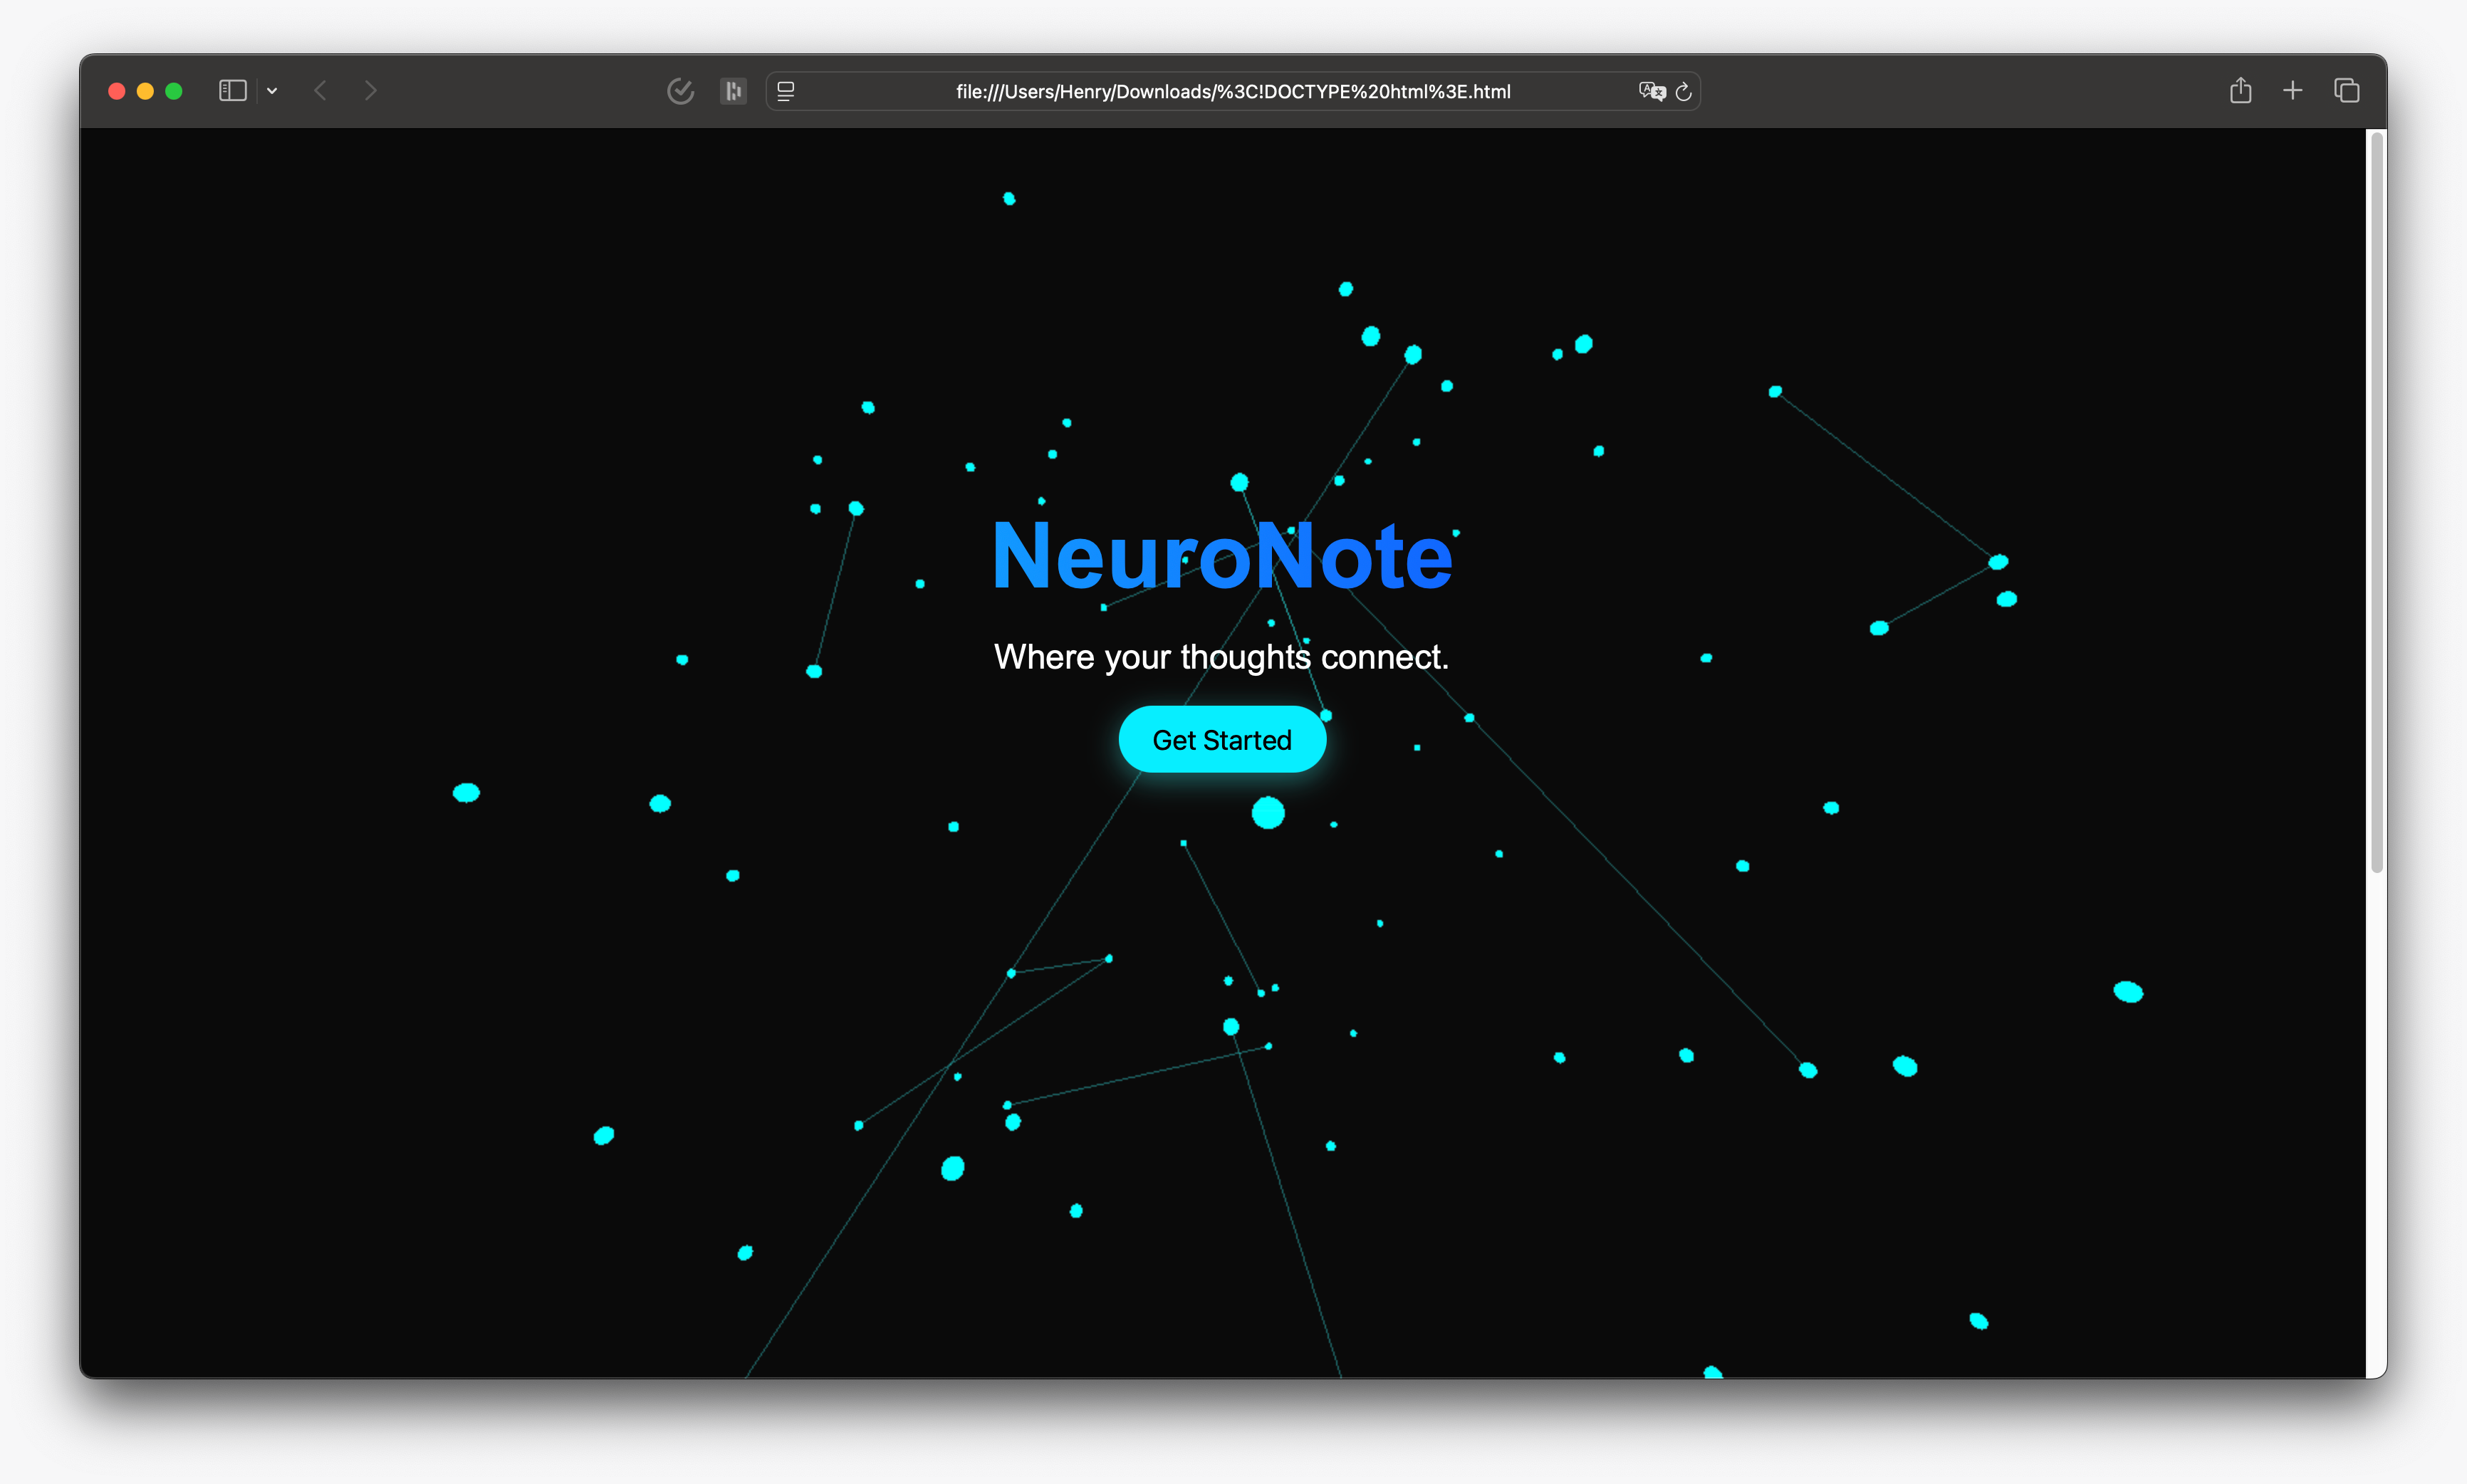
\includegraphics[width=\textwidth]{Diary/32_WC_9-6-25/media/firstLandingPage.png}
        \caption{First prototype of landing page}
    \end{minipage}
    \hfill
    \begin{minipage}[b]{0.48\textwidth}
        \centering
        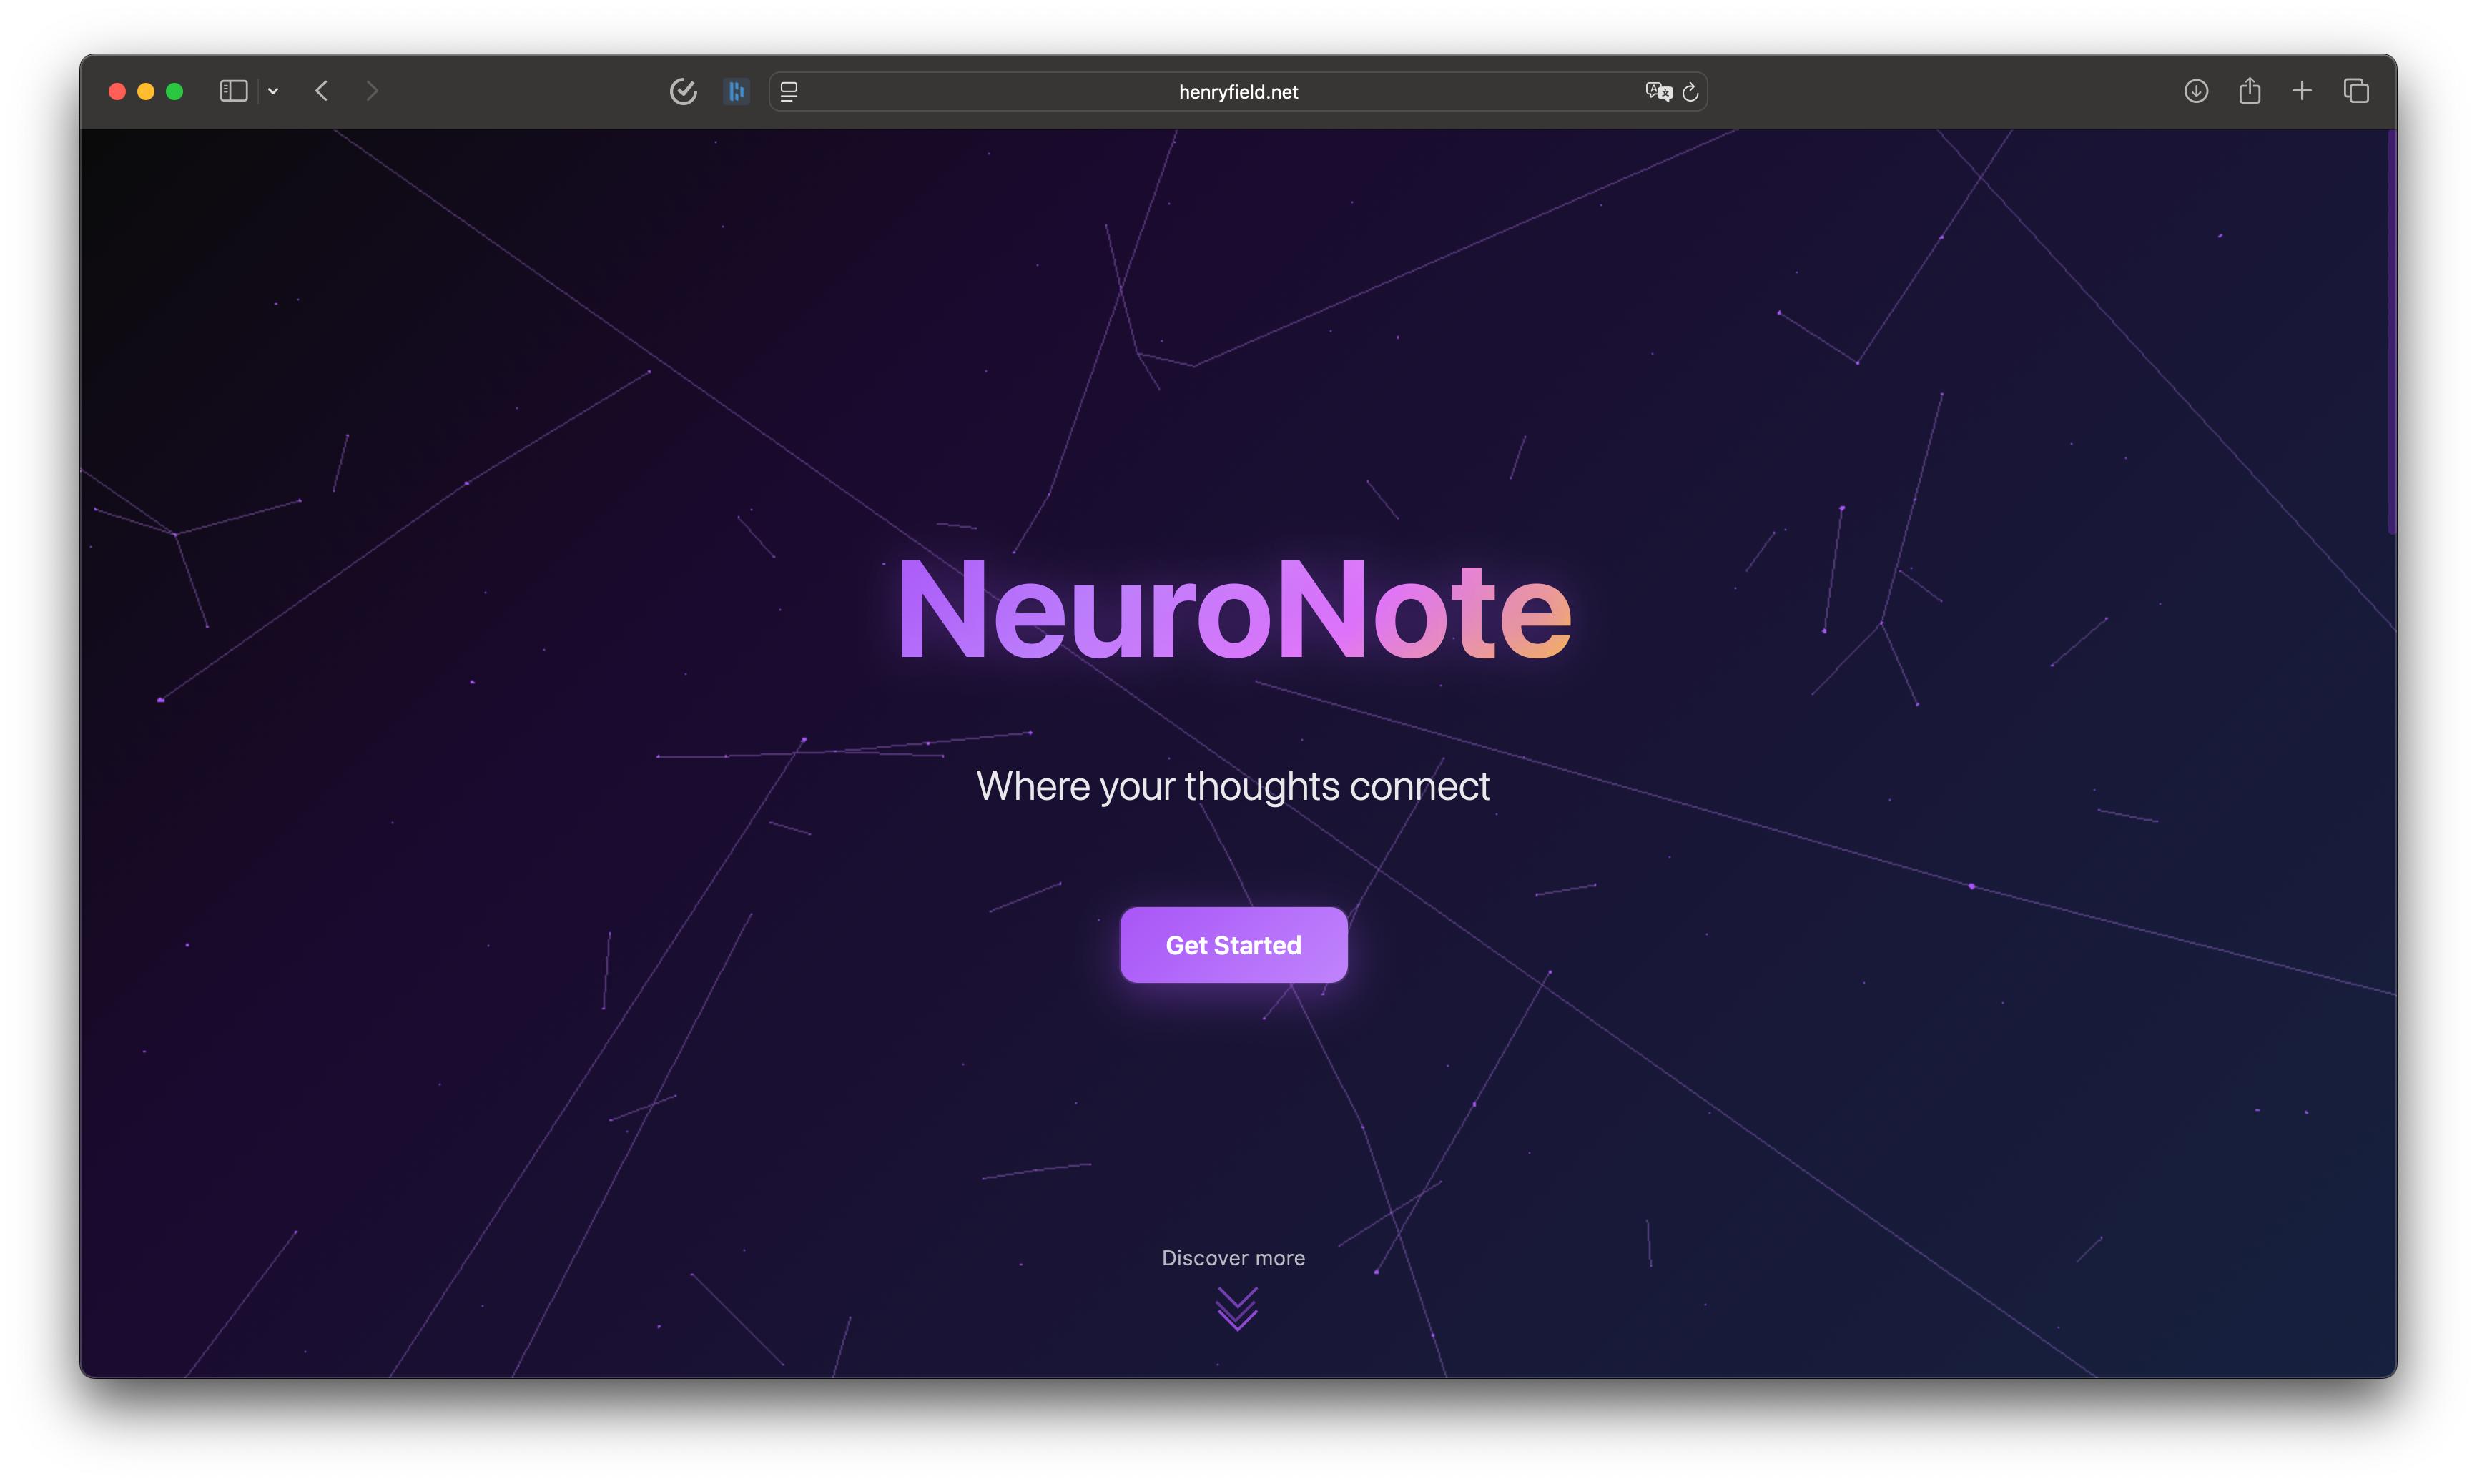
\includegraphics[width=\textwidth]{Diary/32_WC_9-6-25/media/finalLandingPage.png}
        \caption{Final version of landing page}
    \end{minipage}
\end{figure}

\begin{figure}[H]
    \centering
    \begin{minipage}[b]{0.48\textwidth}
        \centering
        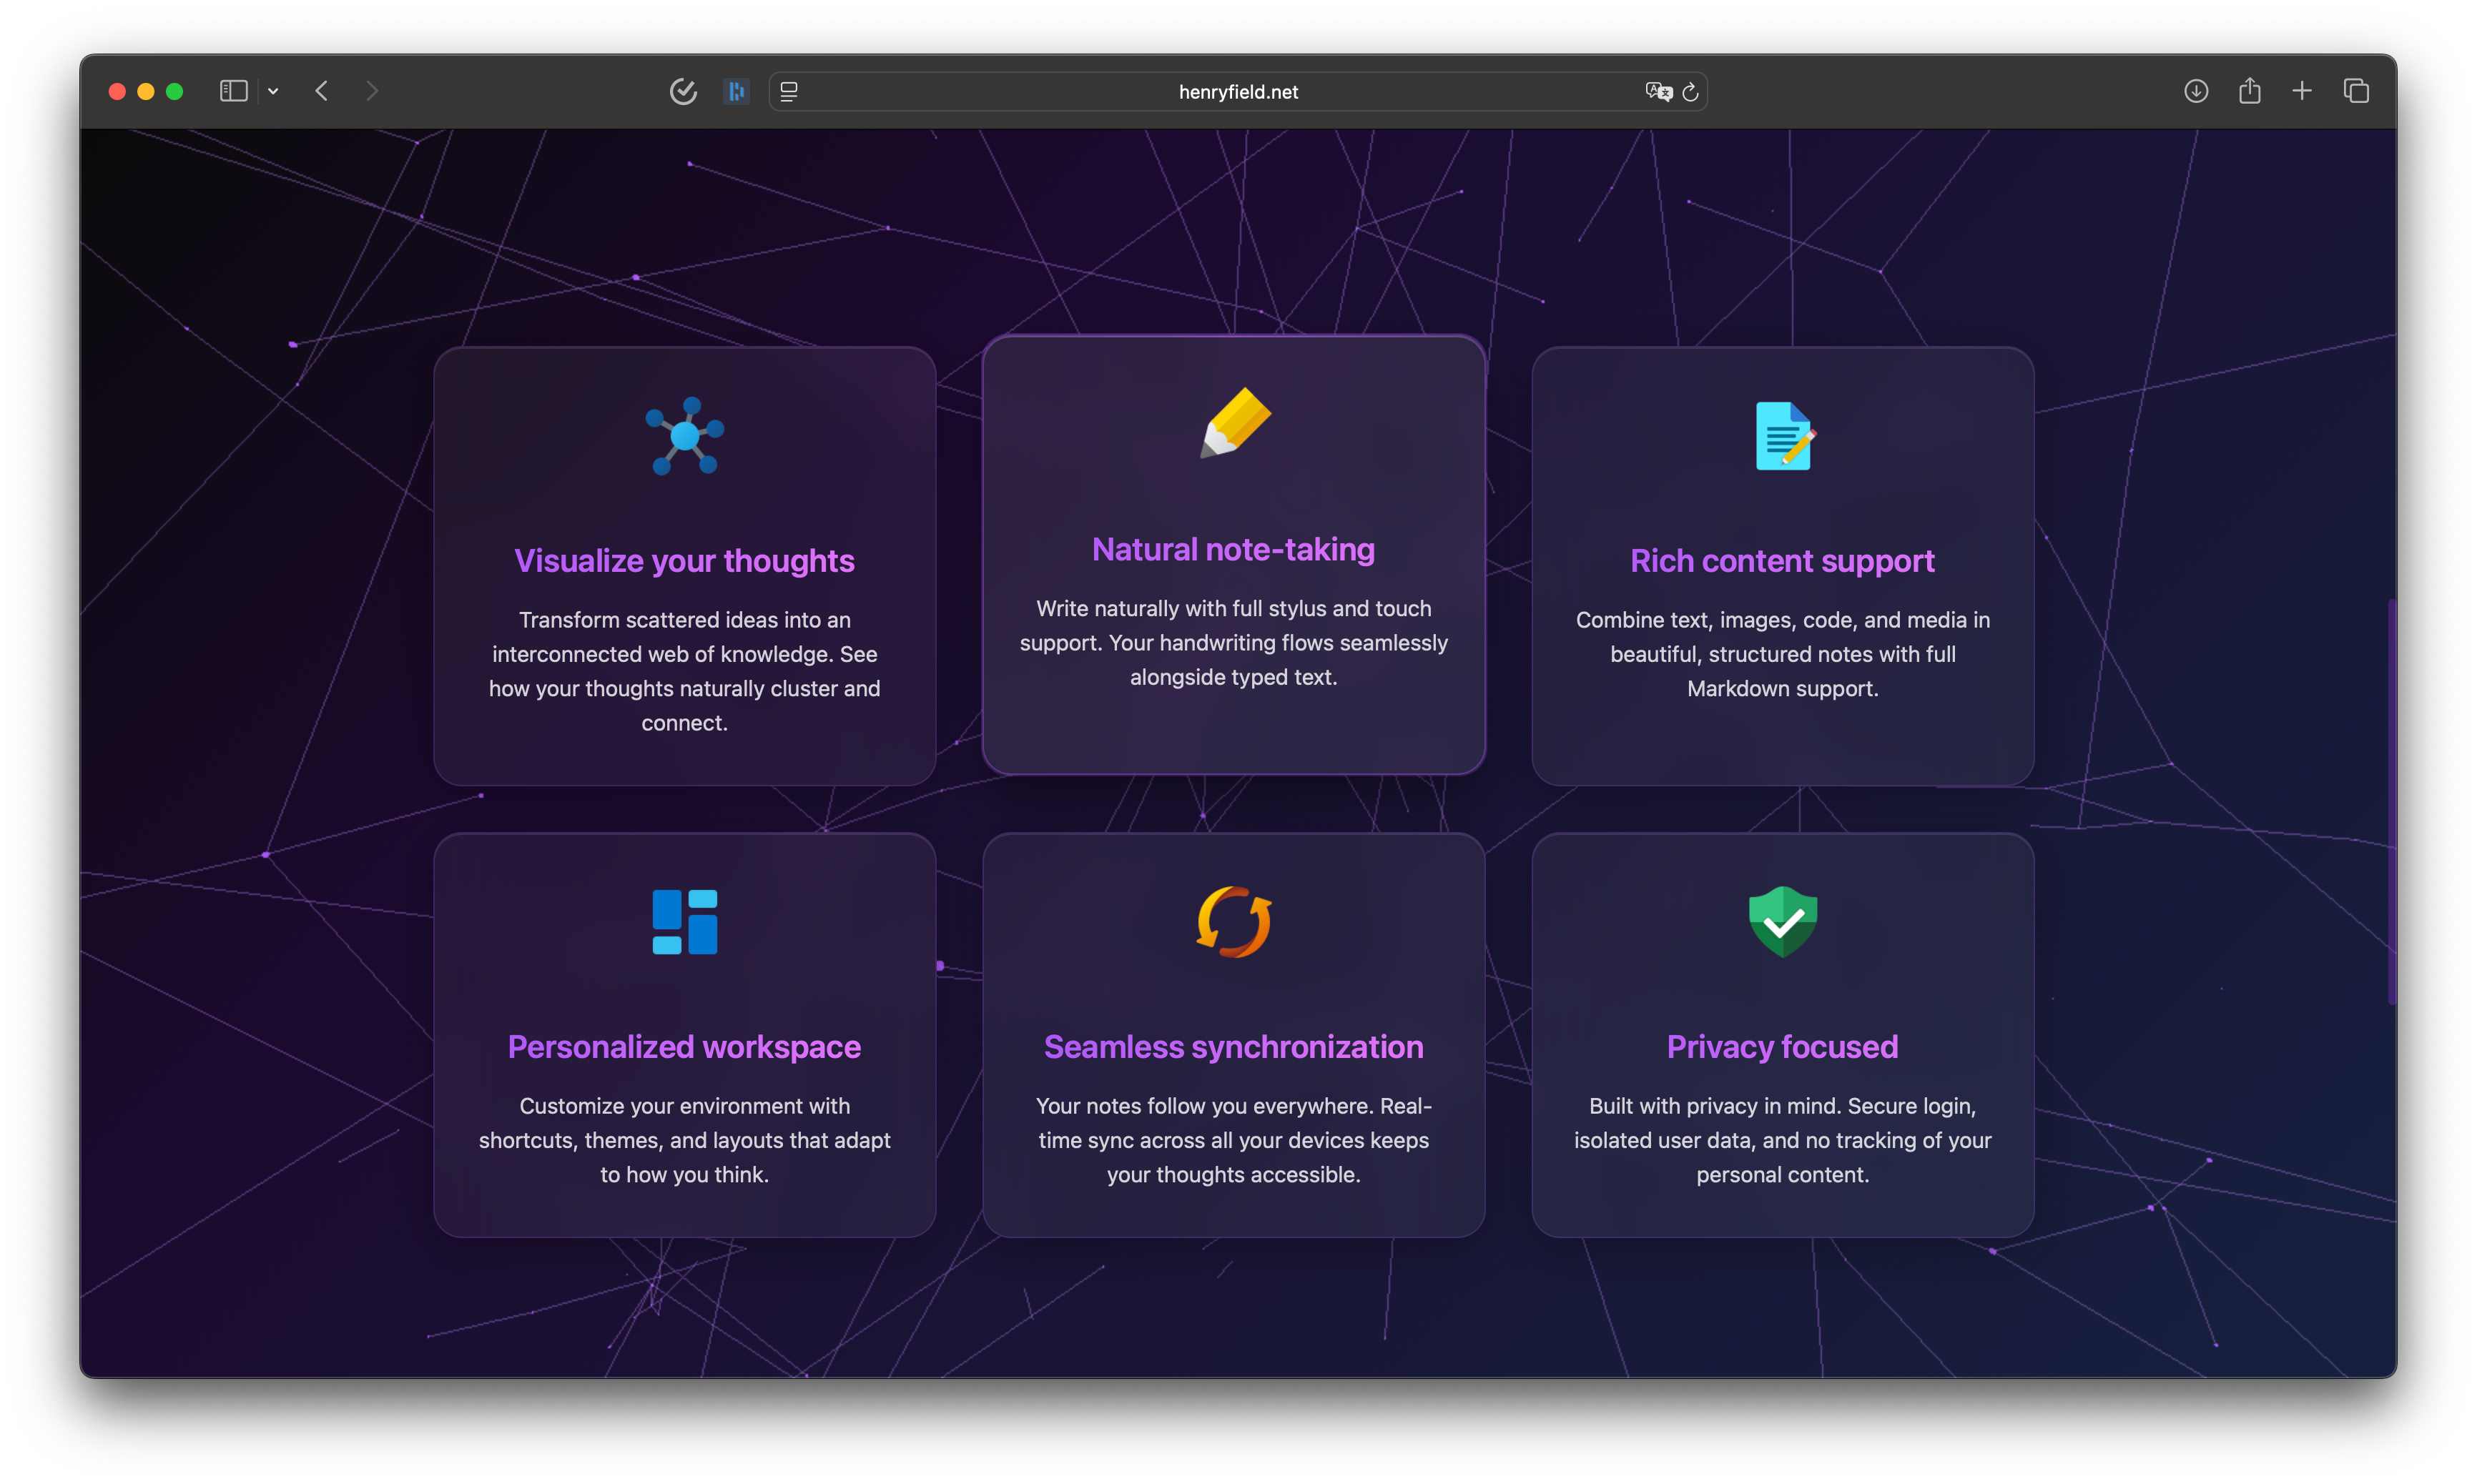
\includegraphics[width=\textwidth]{Diary/32_WC_9-6-25/media/landingDetail.png}
        \caption{Project details section}
    \end{minipage}
    \hfill
    \begin{minipage}[b]{0.48\textwidth}
        \centering
        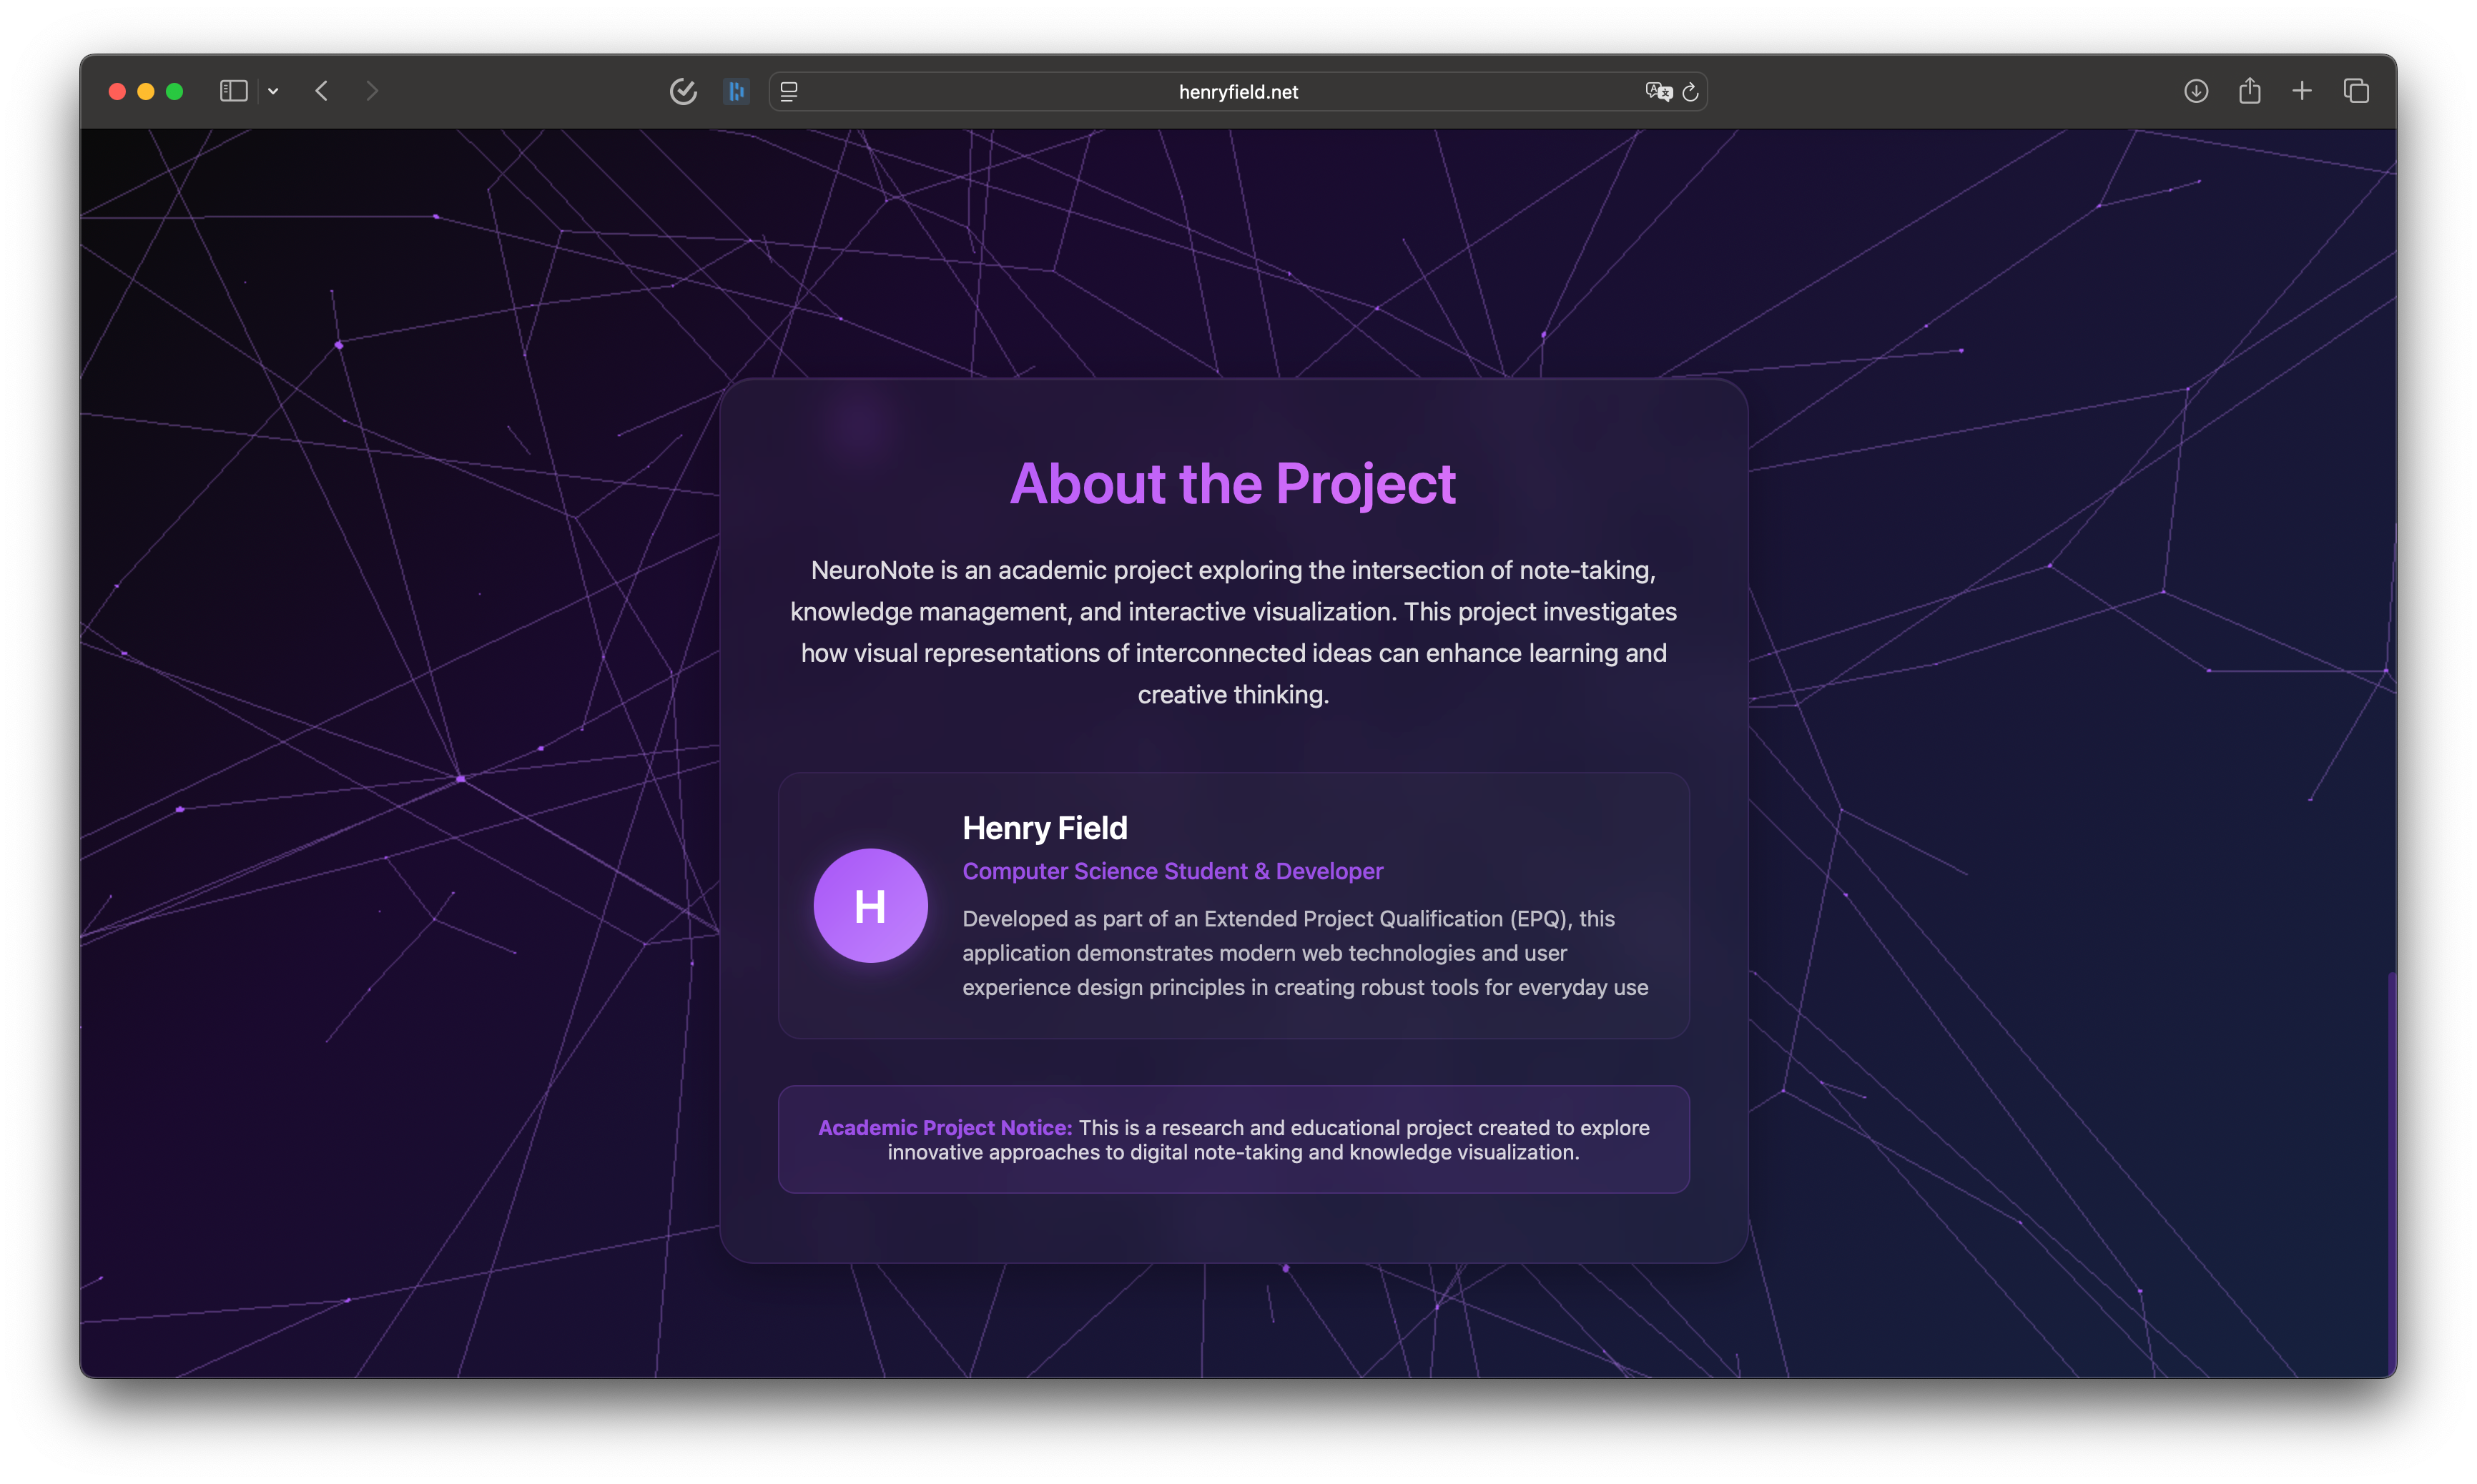
\includegraphics[width=\textwidth]{Diary/32_WC_9-6-25/media/landingAbout.png}
        \caption{About section}
    \end{minipage}
\end{figure}

After creating my landing page I noticed that the user-flow of welcome page -> login -> main application felt 'clunky' as there was two discrete changes in the UI design (one for each step as I had iterated throughout my EPQ Journey). Whilst the change leading into the main notetaking experience is intentional and serves functional purposes I wanted to update my login/registration page to reflect the new graph, simulation design. Please see the final product below.

\begin{figure}[H]
    \centering
    \begin{minipage}[b]{0.48\textwidth}
        \centering
        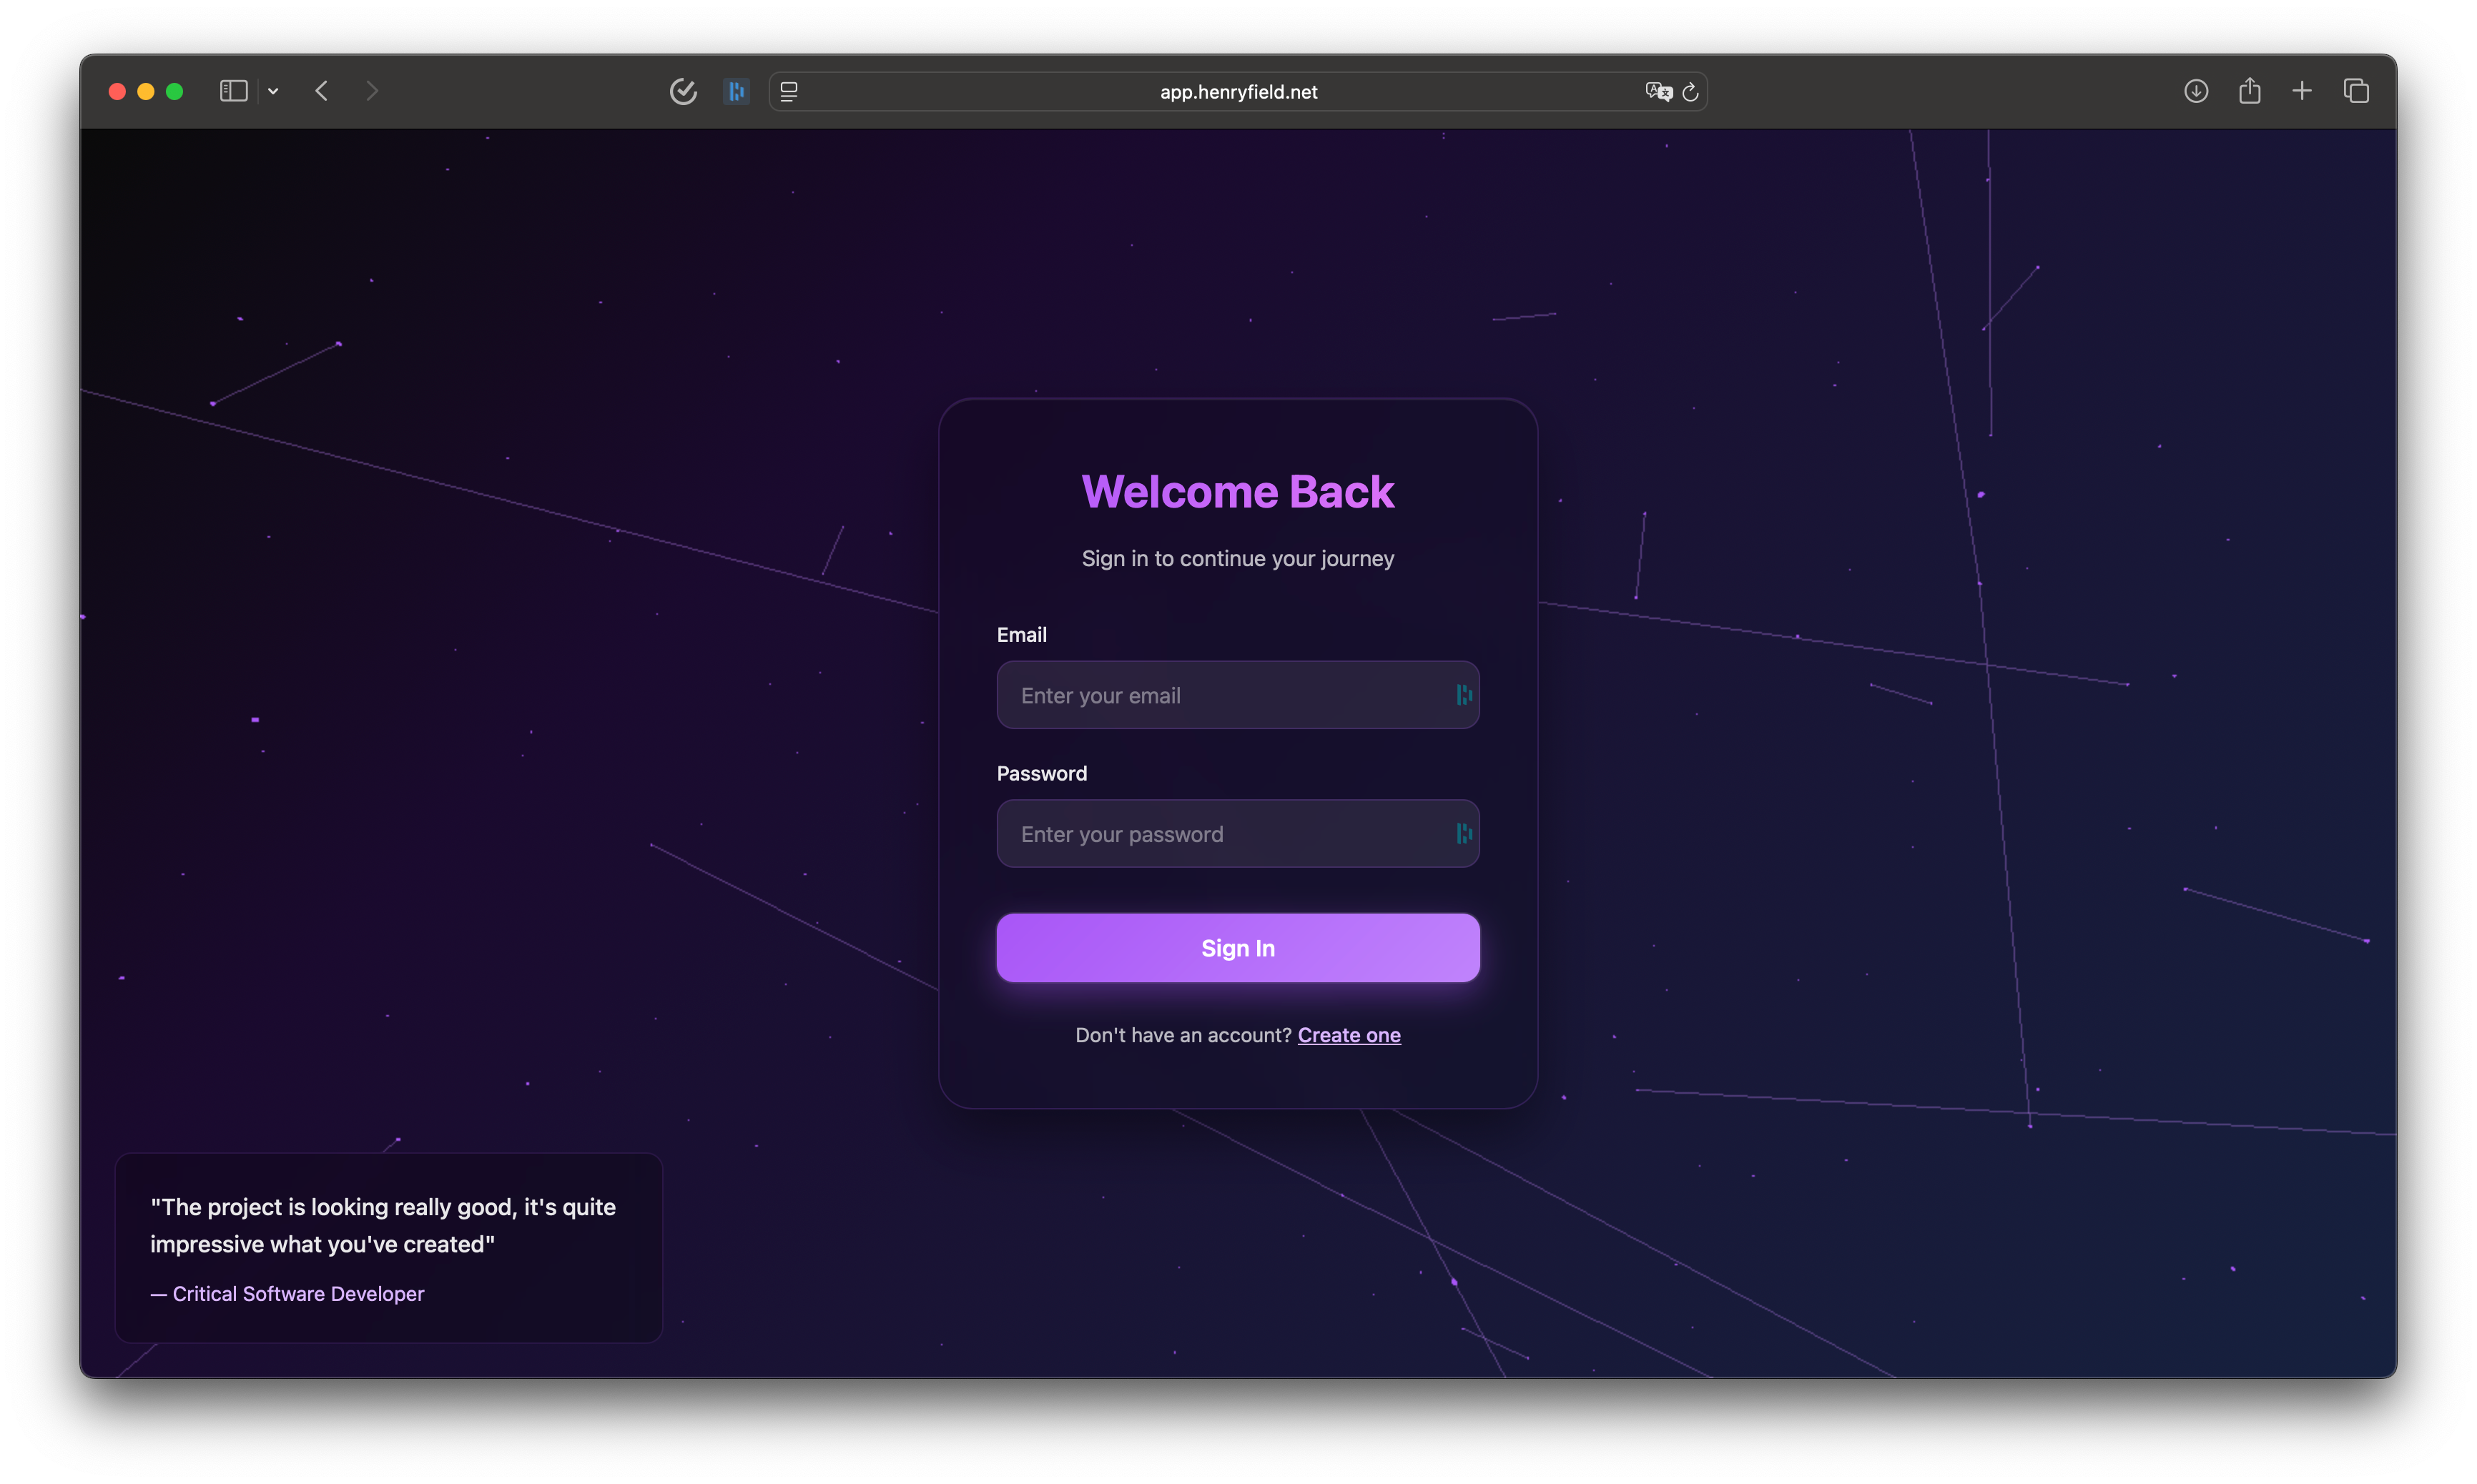
\includegraphics[width=\textwidth]{Diary/32_WC_9-6-25/media/loginPage.png}
        \caption{Login page}
    \end{minipage}
    \hfill
    \begin{minipage}[b]{0.48\textwidth}
        \centering
        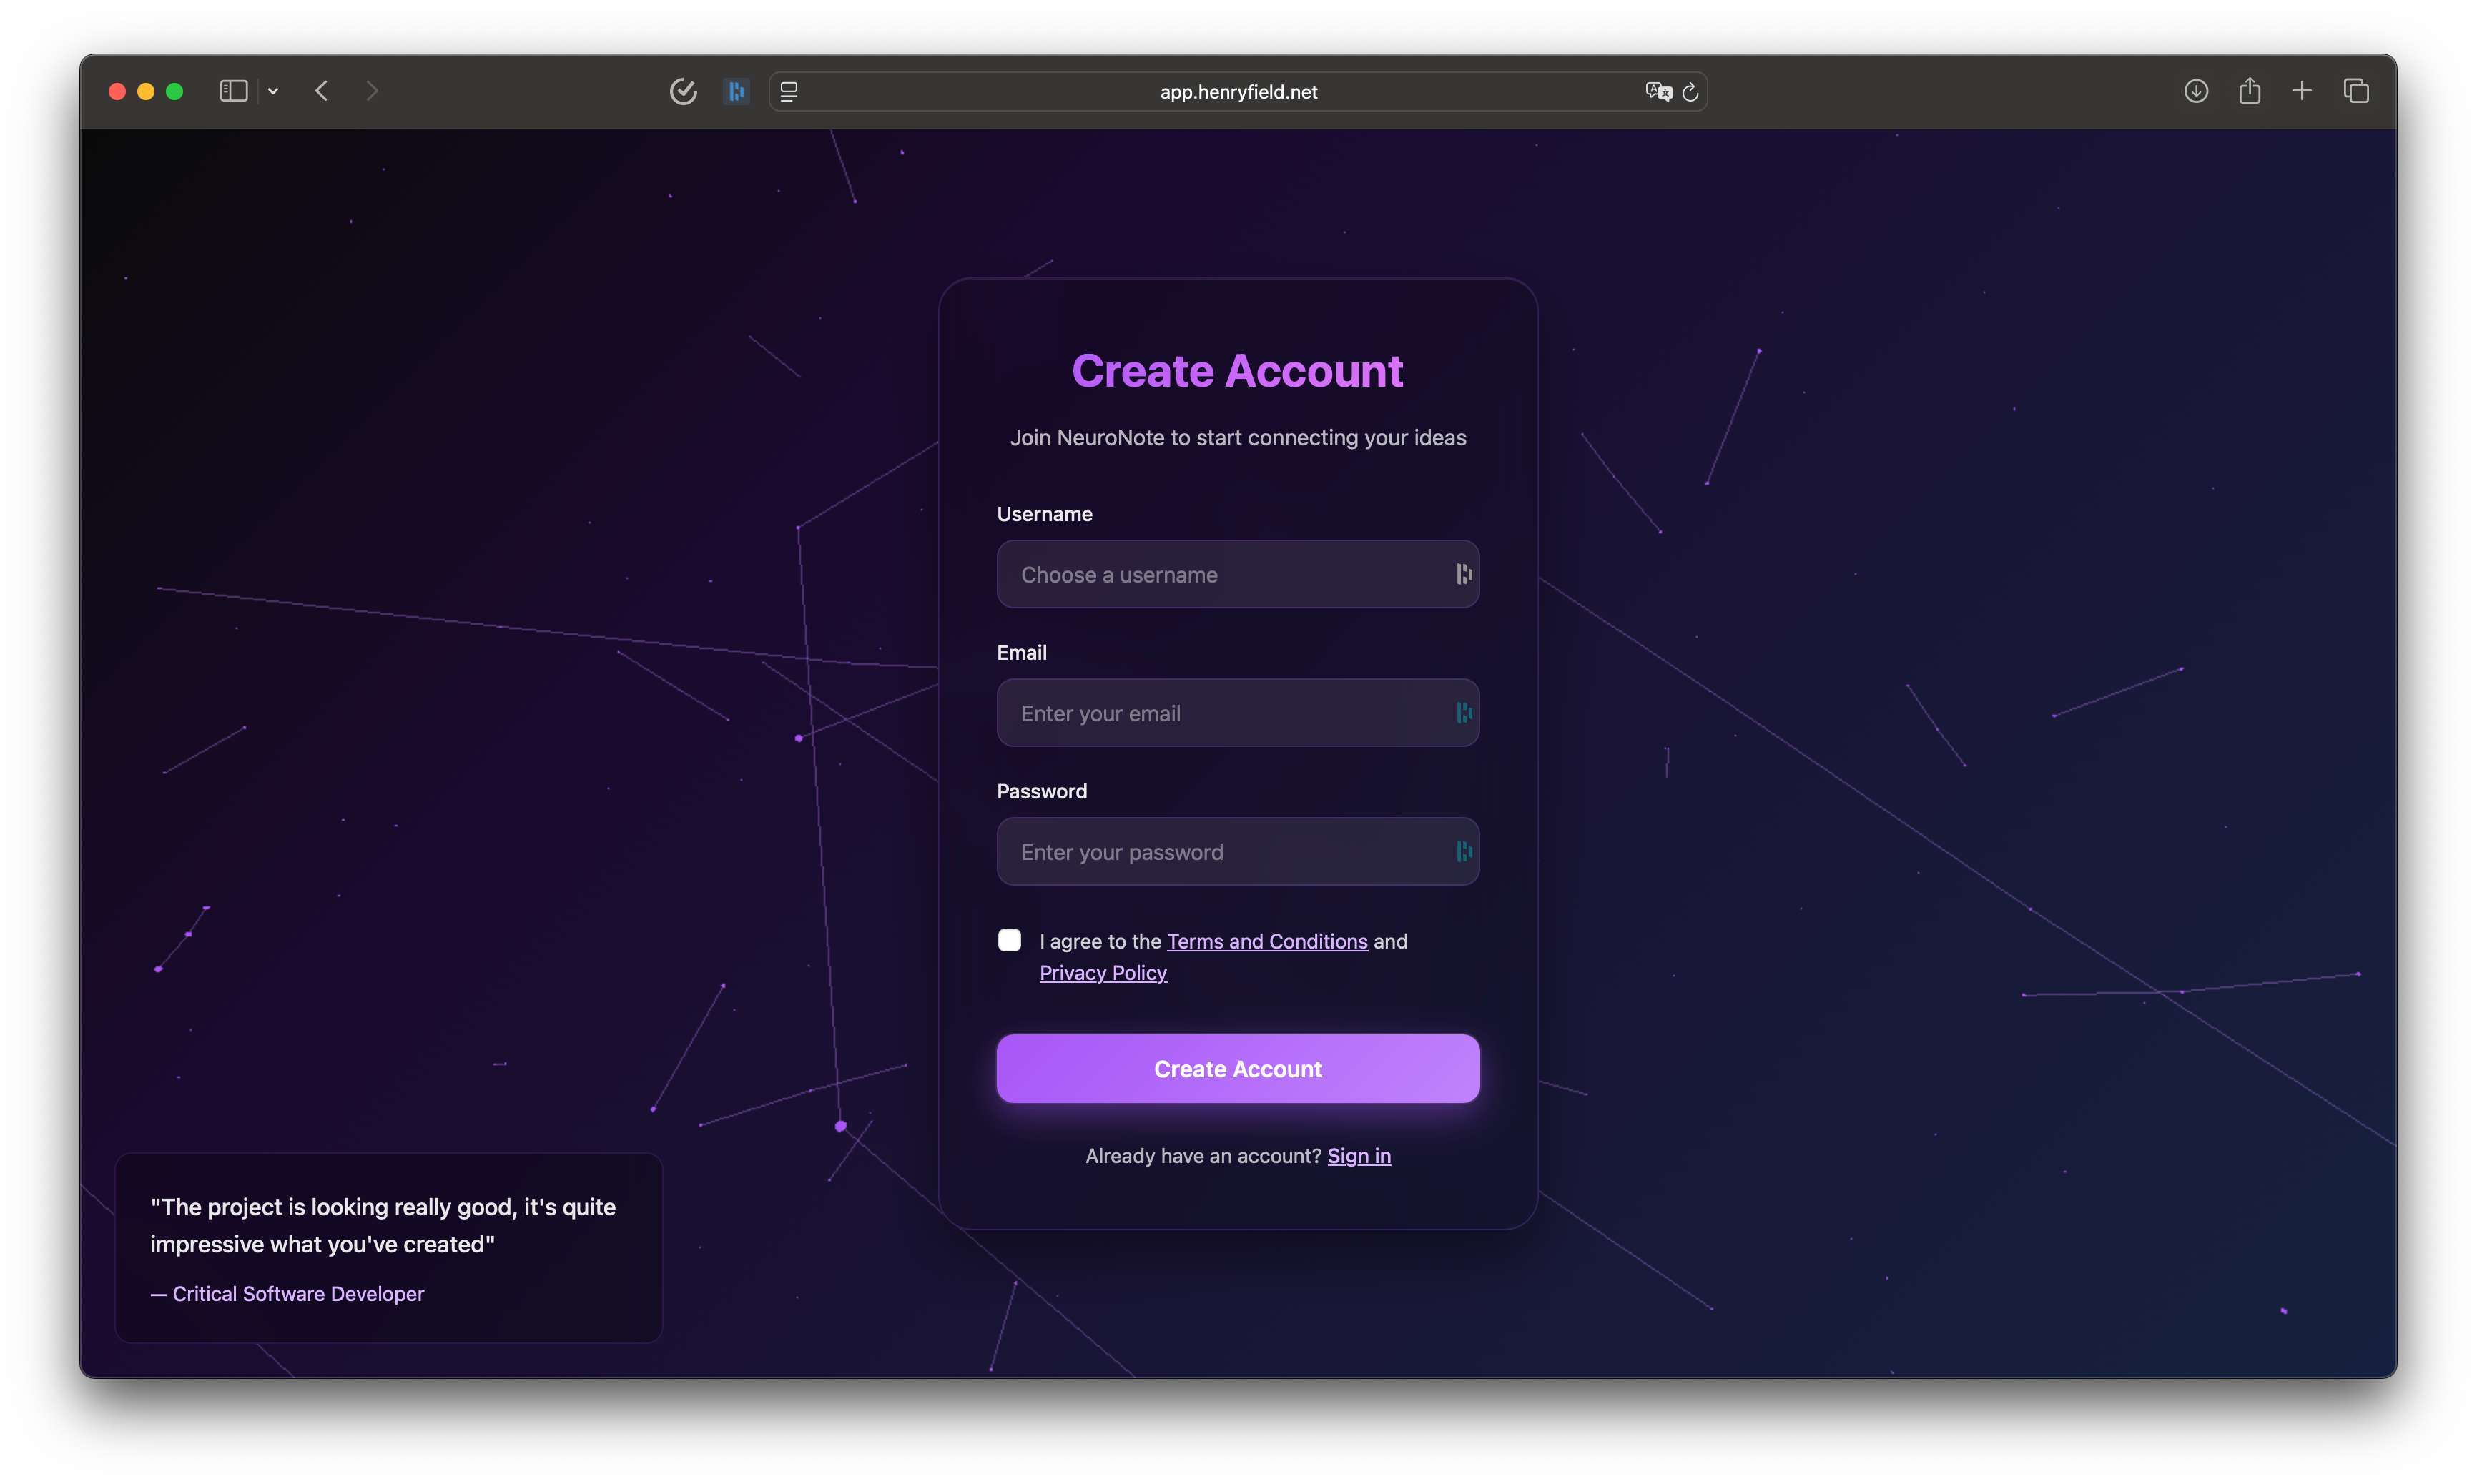
\includegraphics[width=\textwidth]{Diary/32_WC_9-6-25/media/registrationPage.png}
        \caption{registration page}
    \end{minipage}
\end{figure}

I did experiment with updating the rest of the UI with this starry, glassy aesthetic however found this made text less legible and features more confusing. Due to the functionality decreases I have chosen to roll this back and keep my main application UI unchanged despite my personal liking to this concept. Some peers I asked also shared the same opinions. Please see my mock design below:

\begin{figure}[H]
    \centering
    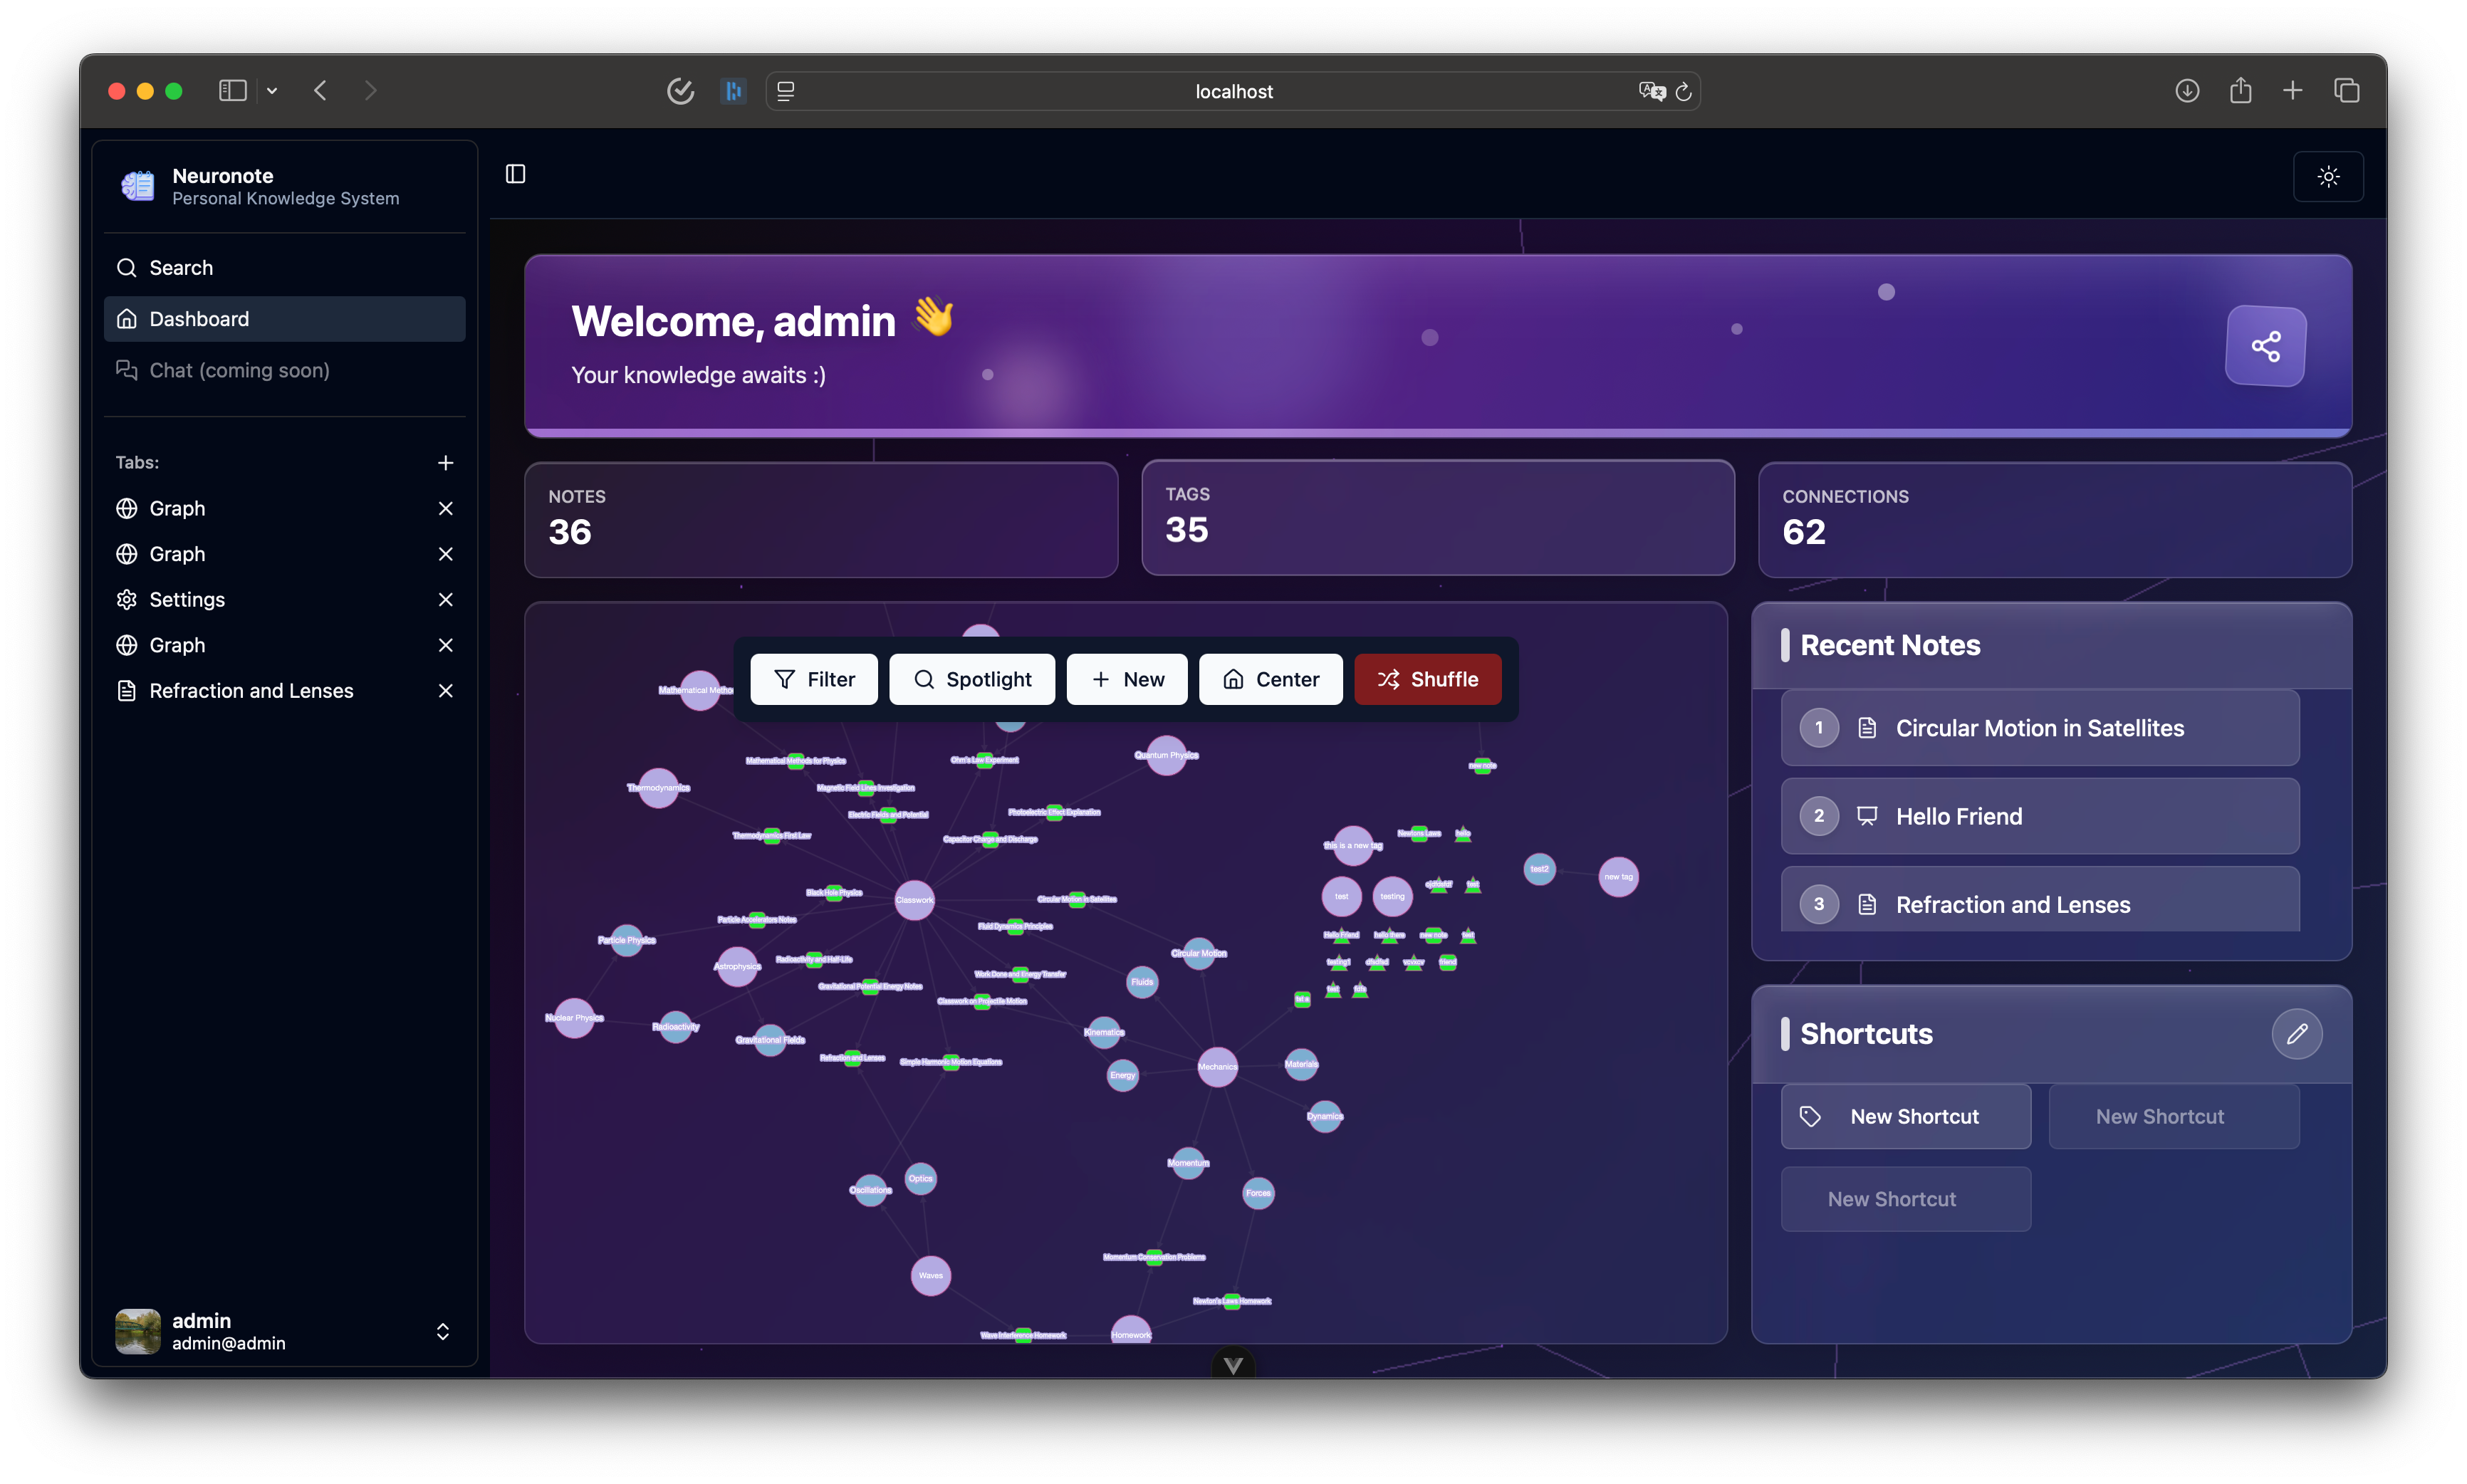
\includegraphics[width=0.8\textwidth]{Diary/32_WC_9-6-25/media/GlassyDashboard.png}
    \caption{Mockup of glassy dashboard}
\end{figure}

Whilst exploring and testing these pages on a variety of devices however I noticed that the load times were quite poor. To quantify this I visited Google's page speed insights service which gave my site scores in a number of categories. Due to research and implementation of accessibility tools I scored well (achieving 81) in the accessibility category and only losing marks due to now unused images not having text descriptions however, my performance score was 36 which is very poor. Whilst a lower score can be expected for webapps such as this when compared to much simpler 'static' websites this poor score was due to an overly large number of code 'packages' being served from a slow server. 

\begin{figure}[H]
    \centering
    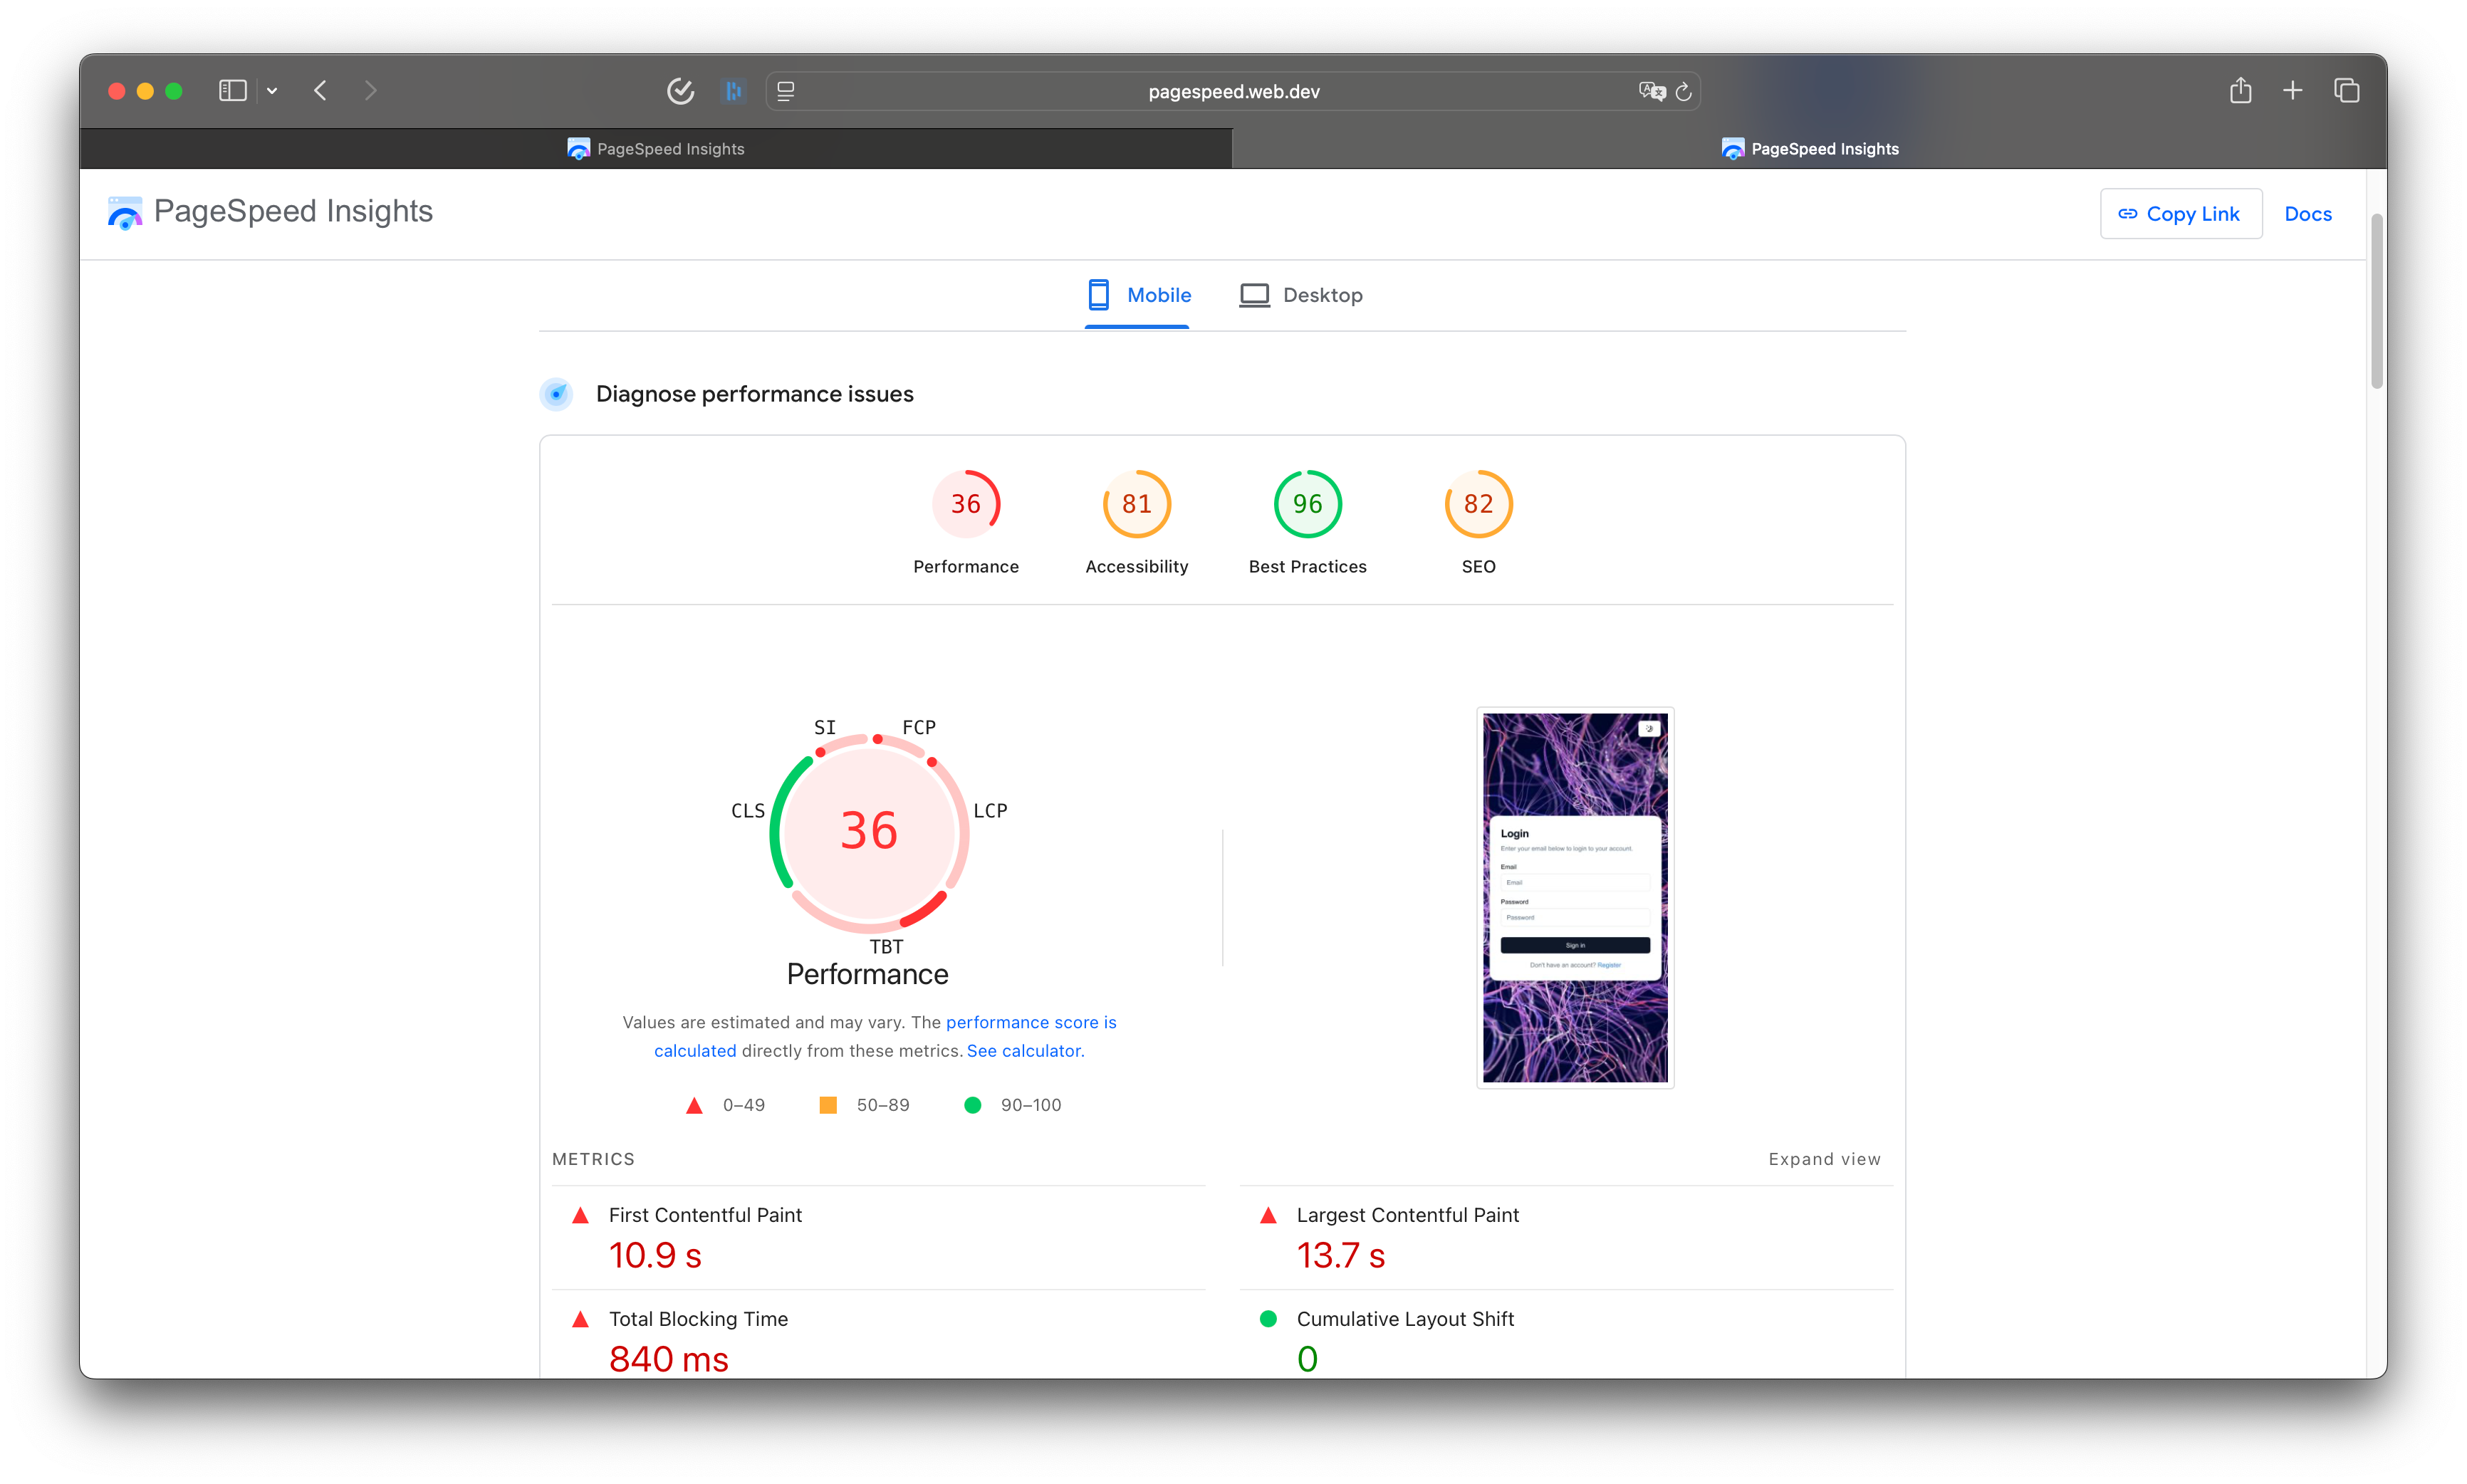
\includegraphics[width=0.8\textwidth]{Diary/32_WC_9-6-25/media/beforeStat.png}
    \caption{Google's performance report}
\end{figure}

After doing some testing on where the slowdowns originated it turns out that some of the software libraries I use for functionality (such as the mathematical Katex library) were sending much more code/features than were actually required and that these large files weren't being cached by my Cloudflare CDN (content delivery network which takes note of commonly requested data such as the welcome page and caches it in all of Cloudflare's very fast worldwide datacentres rather than having to have my Raspberry Pi at home relay the information which would take far longer) and had to take the slower route from my house. My testing of load times hadn't caught this as once my computer had initially loaded that data it was kept for future browsing session and that initial load also didn't take very long due to my close proximity to the server (which was just next to me).

To solve these performance issues I took two approaches: firstly I went through each and every library I am using and made sure they were 'tree shakeable', this means that when I 'build' my code into the final distributable software that my server sends to user it can intelligently remove any library code that isn't used, massively reducing the code required by each client. In fact having completed this process I brought my 'package size' from 5000kB down to just 700kB - a huge improvement. Secondly I switched from hosting the frontend code on my server to entirely running on Cloudflare's CDN, whilst all of the functional backend (and backup frontend) run on my Pi, all users now have access to a lightening fast copy of my webapp. Finally, I removed all the unused images and assets previously identified by Google Insights.

With these performance updates complete I retested my project and saw my scores jump up to an incredible 97 in performance - a huge improvement and something I am very proud of achieving.

\begin{figure}[H]
    \centering
    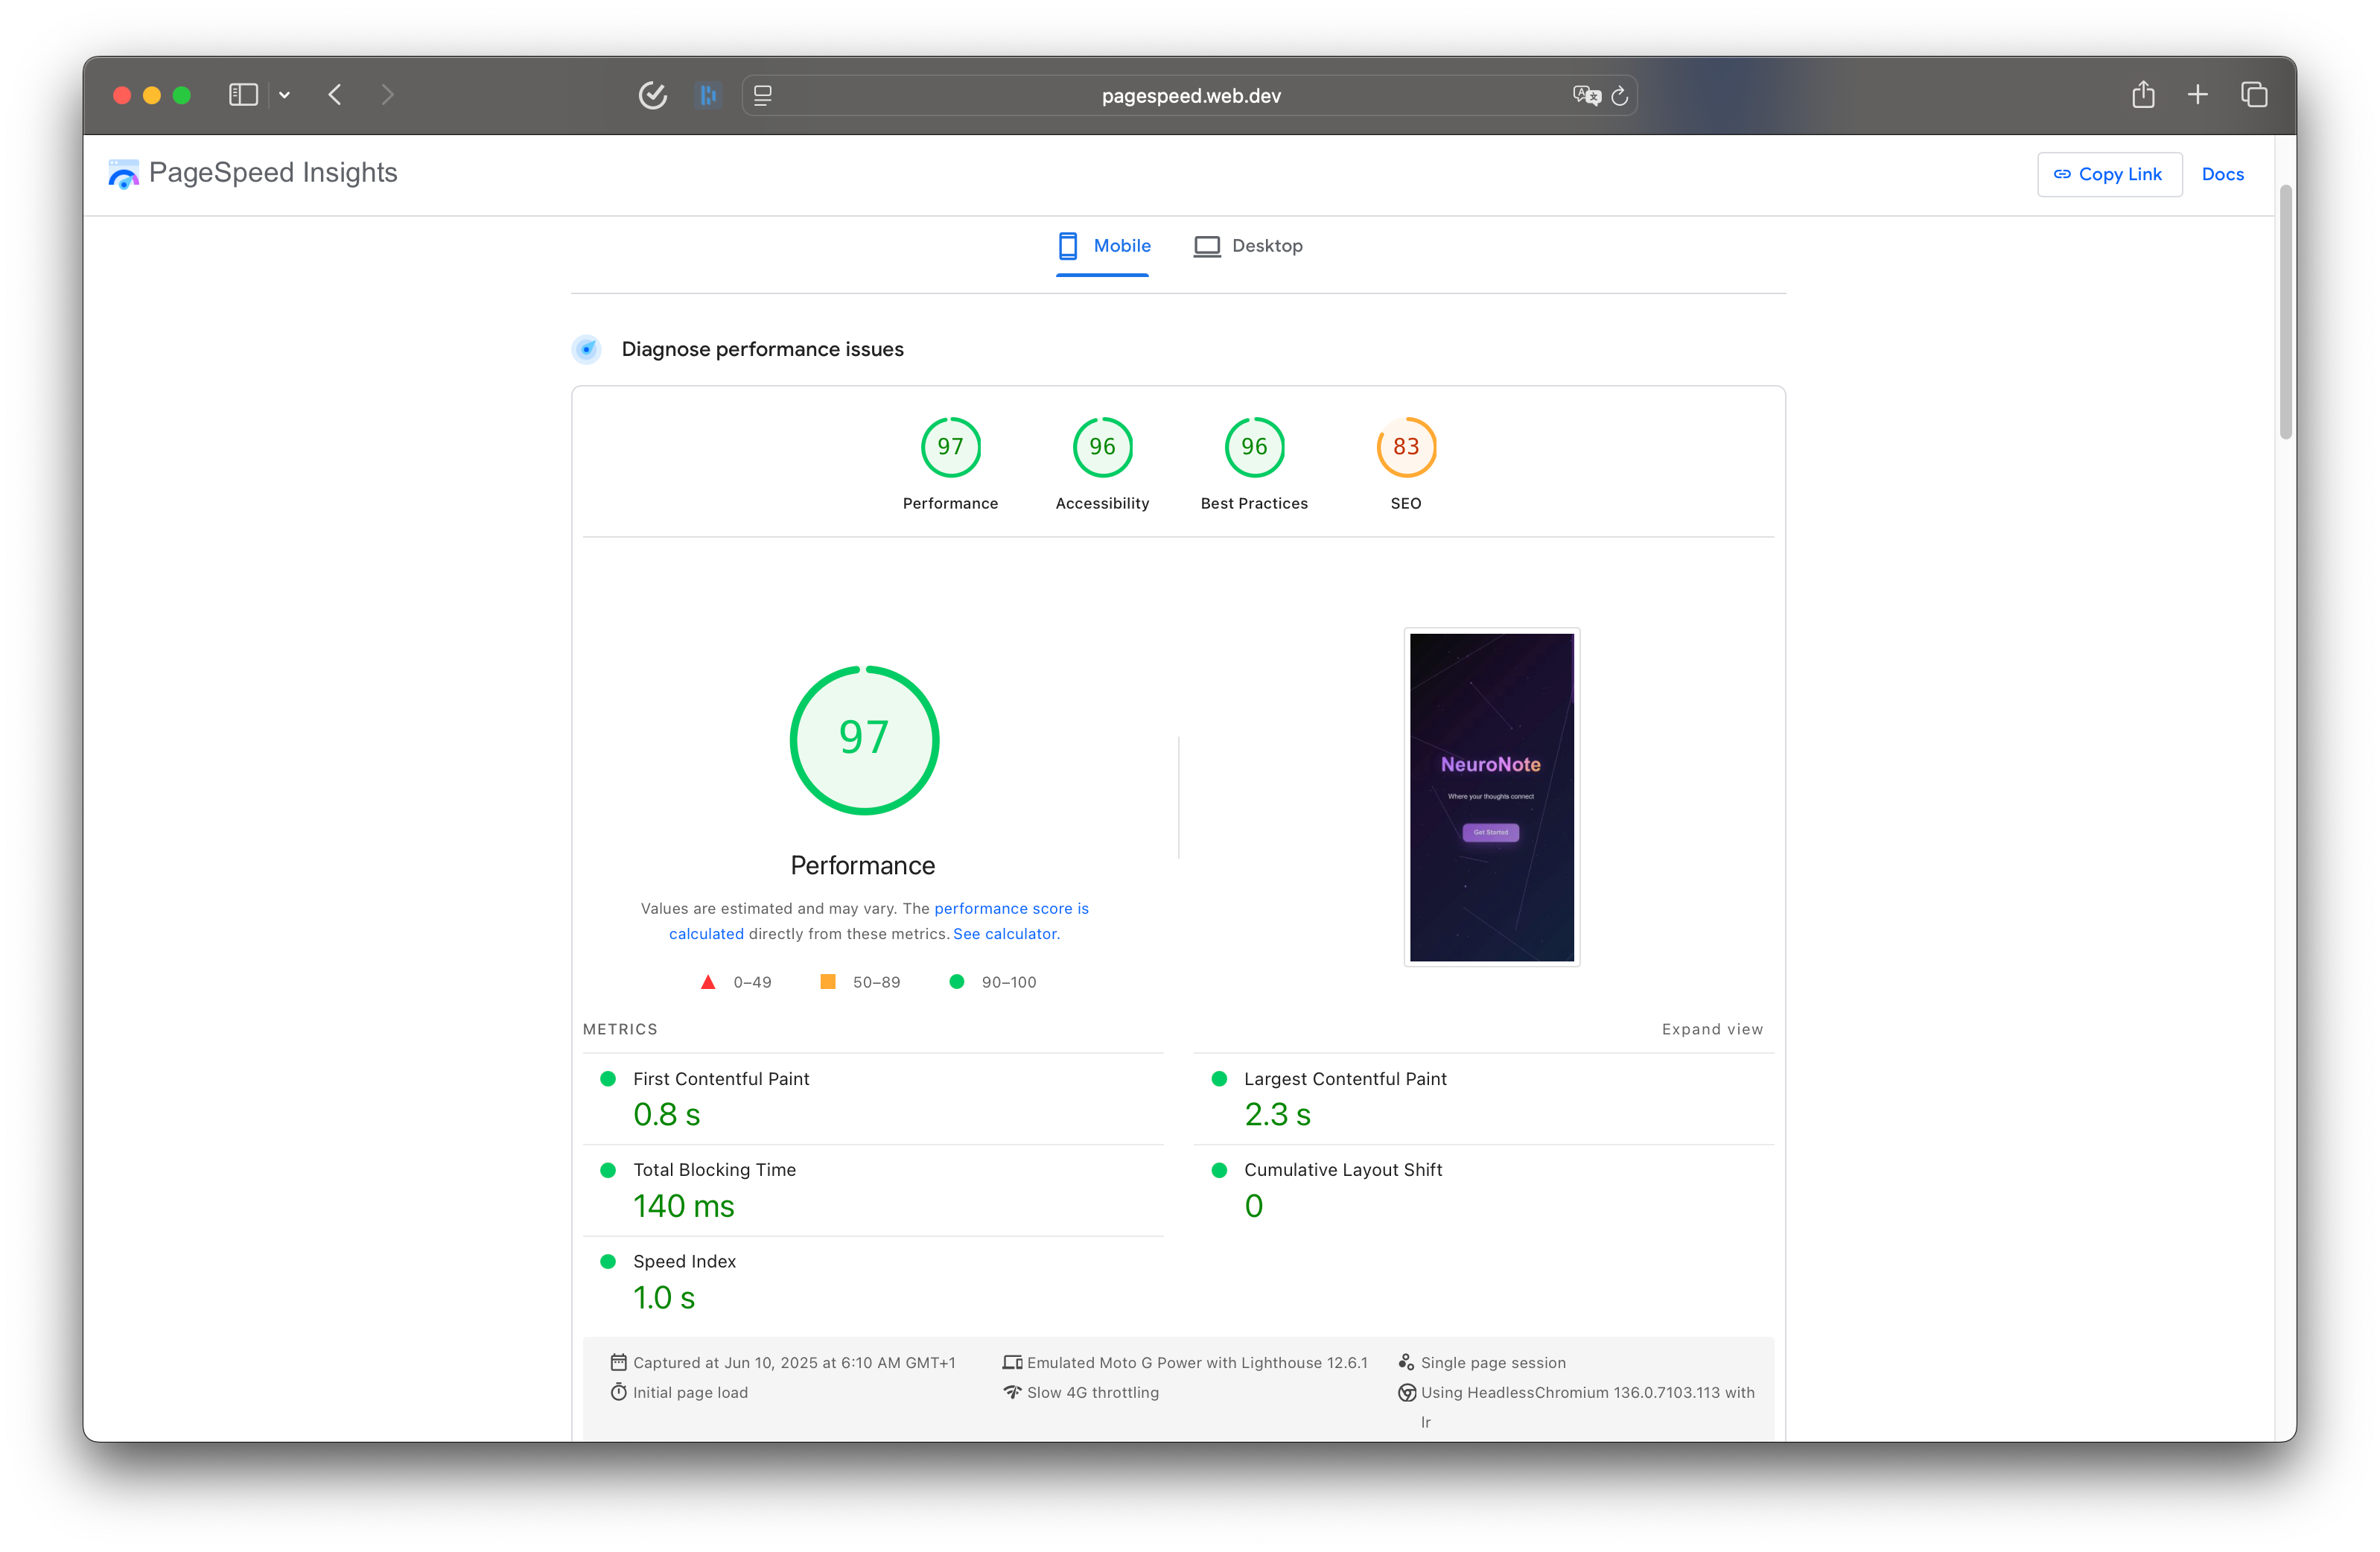
\includegraphics[width=0.8\textwidth]{Diary/32_WC_9-6-25/media/afterStat.png}
    \caption{Google's new performance report}
\end{figure}

Lastly this week I found myself unable to tell if my project was operating smoothly or if my users would be facing errors so I researched a variety of technique to get instant reports if something goes wrong. I settled on using a platform called Uptime robot (whilst I could build something myself, should I lose internet / have a power cut at home it would render the system pointless). I built an API health check page on my server which Uptime Robot would attempt to connect to every 5 minutes, if the connection failed for whatever reason. I am sent an email notification and an SMS (text) message with the details so that I can resolve them. Tools such as this are crucial in 'professional' software environments and by integrating them into my project now I am setting myself up for future success. (spoiler: it has already proven very useful as later mentioned)

\subsection*{Plans for next week:}
Next week I aim to finish up my project before releasing to my wait list the week after! I will be focusing on testing and bug fixing as well as creating a user guide to help new users get started with my project. I also aim to create a short promotional video to help advertise my project on social media.
